% 由原 ICIP 中文稿精简；保留历史结果，不代表新增实验。
\documentclass{article}
\usepackage{spconf,amsmath,amssymb,graphicx,booktabs,xcolor,url}
\usepackage{balance}
\usepackage{xeCJK}
\setCJKmainfont{SimSun}[AutoFakeBold=true,ItalicFont=KaiTi]
\setCJKsansfont{SimHei}
\graphicspath{{assets/}}
\renewcommand{\topfraction}{0.92}
\renewcommand{\dbltopfraction}{0.92}
\renewcommand{\textfraction}{0.08}
\title{低频替换与校准：扩散式时空融合推理期校正的诊断性研究}
\name{匿名作者}
\address{匿名单位}
\begin{document}
\ninept
\maketitle

\begin{abstract}
单步扩散时空融合（STF）降低了采样开销，却可能保留低频时间偏差。我们用参考影像与粗观测构造锚定目标，替换预测的低频分量，无须拟合参数，仅需一次网络评估。二十种推理期变体的历史评测中，该算子相对未校正单步输出使 LGC 稳定期与洪水期 RMSE 分别改善 14.2\% 和 6.4\%；CIA 测试期改善、验证期退化，给出明确的迁移边界。精细与粗糙时间变化的线性诊断（$a=0.544$、$R^2=0.278$）为校准比较提供依据。九骨干训练研究进一步揭示划分间的权衡，以及时间条件门控向近常数的坍缩。这些探索结果支持观测锚定，也限定了其普适性。
\end{abstract}
\begin{keywords}
时空融合, 扩散模型, 低频替换, 推理期校正, 遥感
\end{keywords}

\section{引言}
\label{sec:intro}
扩散式 STF 利用两个粗/细参考对及预测日粗影像，重建该日精细影像。近期方法改进了条件生成~\cite{huang2024stfdiff,zhang2026sastf,zhu2026dpdiff}，但迭代采样仍有较高开销。缩减到单次去噪后，预测的时间变化可能与粗传感器观测不符。

双锚点协议为推理期校正提供了两对参考。逐样本回归、传输或分布对齐尝试拟合粗细关系；另一条路径是直接利用观测变化锚定预测。本文检验两个问题：拟合何时有益，更好的训练能否替代推理期校正？

本文提出无拟合参数的低频替换，并以二十种校正变体和九个训练骨干检验其作用。核心证据同时包括 LGC 增益与 CIA 验证期失败，目标是界定校正机制的适用范围。

\section{相关工作}
\label{sec:related}
STFDiff 通过双流预测器实现扩散式 STF~\cite{huang2024stfdiff}；SA-STF 引入时间对齐与语义自适应融合~\cite{zhang2026sastf}；DPDiff 将双先验接入生成过程~\cite{zhu2026dpdiff}。这些方法改进条件生成，本文则利用双锚点协议已有的观测校正冻结预测，比较拟合校准与直接替换，无须额外精细影像或推理期参数适应。

\section{协议与算子}
\label{sec:method}
\subsection{输入与评价}
输入为 $(F_p,C_p)$、$(F_n,C_n)$ 和 $C_t$，目标精细影像 $F_t$ 不进入推理。冻结骨干含 7.49\,M 参数，一次去噪返回 $x_1$。低通算子 $\mathrm{LP}$ 为高斯滤波（$\sigma=2$），各方法共享校正强度 $\lambda=0.3$。模型使用 $[-1,1]$ 归一化，RMSE 报告于 $[0,1]$。

LGC 每划分 120 个 patch：稳定期验证三元组为 2005-02-14/03-02/04-03，洪水期测试为 2004-12-28/2005-01-13/01-29；CIA 验证与测试分别含 126、168 个 patch。表中复用历史评测；权重来源、采样设置及旧指标口径仍需核验，因此不作为同协议外部 SOTA 超越证据。

\subsection{低频替换与拟合校准}
校准在样本自身参考上拟合 $\mathrm{LP}(F_n-F_p)\approx a\,\mathrm{LP}(C_n-C_p)+b$。前锚点目标为
\begin{equation}
T_p=\mathrm{LP}(F_p)+a\,\mathrm{LP}(C_t-C_p)+b,
\label{eq:target}
\end{equation}
再执行
\begin{equation}
x_{\mathrm{out}}=x_1-\lambda\bigl(\mathrm{LP}(x_1)-T\bigr).
\label{eq:proj}
\end{equation}
历史替换实现取 $T=T_p$、固定 $a=1,b=0$，省去逐样本拟合，在保留骨干细节估计的基础上加入低频校正。双锚变体构造 $T_n=\mathrm{LP}(F_n)+a\,\mathrm{LP}(C_t-C_n)-b$，对 $T_p,T_n$ 平均或逆方差加权。

二十个选定配置覆盖 OLS、TLS、Deming、Huber、岭、变化加权、逆方差、跨度归一化及恒等估计，并考察高斯、Haar、引导和双尺度投影，以及分布对齐、自适应强度与两步不动点。该集合并非九种估计器与四种投影的完整笛卡尔积。表~\ref{tab:operators} 固定 $\lambda=0.3$；图~\ref{fig:gain} 的扩展配置与这一比较分别解释。

\begin{table*}[t]
\centering
\caption{冻结项目权重的历史校正结果。RMSE 于 $[0,1]$，共享 $\lambda=0.3$；横线表示原对应表未报告该项，粗体为各列最小值。}
\label{tab:operators}
\begin{tabular}{lcccc}
\toprule
 & \multicolumn{2}{c}{LGC，每划分 120 patch} & \multicolumn{2}{c}{CIA，126/168 patch}\\
\cmidrule(lr){2-3}\cmidrule(lr){4-5}
方法 & 稳定期（验证） & 洪水期（测试） & 验证 & 测试\\
\midrule
历史十步采样器（10 NFE） & 0.02972 & 0.02161 & 0.02716 & 0.02777\\
Fixed-1（1 NFE） & 0.02815 & 0.02053 & 0.02785 & 0.02741\\
源域校准 & 0.02577 & 0.01977 & -- & --\\
逐样本 OLS & 0.02810 & 0.01897 & 0.02776 & 0.02742\\
Huber & -- & -- & 0.02780 & 0.02722\\
岭收缩 & 0.02787 & \textbf{0.01896} & 0.02769 & 0.02737\\
门控校准 & 0.02724 & 0.01943 & \textbf{0.02709} & 0.02677\\
低频替换 & \textbf{0.02416} & 0.01921 & 0.02855 & \textbf{0.02659}\\
\bottomrule
\end{tabular}
\end{table*}

\subsection{架构与训练变体}
\label{sec:arch}
九骨干研究包括 base、三种损失变体（低频、高频及逐波段加权）、四种架构变体及差分监督。架构分别加入显式时间差分（$+0.015$\,M 参数）、噪声时间条件化 sigmoid 门控（$+0.016$\,M）、多尺度条件重注入及三者组合；关闭分支时已检查与原预测器输出差值为零。

差分监督惩罚 $\mathrm{LP}(x_0)-\mathrm{LP}(F_p)$ 偏离 $0.54\,\mathrm{LP}(C_t-C_p)$。历史配方为十个 LGC 三元组、1,200 个 patch，名义预算 40 轮，Adam 学习率 $2\times10^{-4}$，200 步 warm-up、余弦衰减及范数 1.0 的梯度裁剪；batch 为 2，全精度，验证噪声固定。名义预算与实际 checkpoint 阶段、独立评测设置分别记录。

\section{实验结果}
\label{sec:exp}
\subsection{LGC 增益与 CIA 边界}
相对 Fixed-1，低频替换使 LGC 稳定期和洪水期 RMSE 分别改善 14.2\% 和 6.4\%（表~\ref{tab:operators}）。历史逐 patch Wilcoxon 检验分别为 $p=2.1\times10^{-21}$、$7.4\times10^{-17}$，99\% 和 86\% 的 patch 改善。这是探索性的空间比较，不替代独立事件或多训练种子证据。OLS 与岭收缩的洪水期误差更低，替换则在稳定期最强。

CIA 上，替换相对 Fixed-1 改善测试 RMSE 3.0\%，却使验证 RMSE 退化 2.5\%。门控校准在验证期最优，替换在测试期最优。不同划分的反向变化限定了统一校正算子的适用范围。

\begin{figure}[t]
\centering
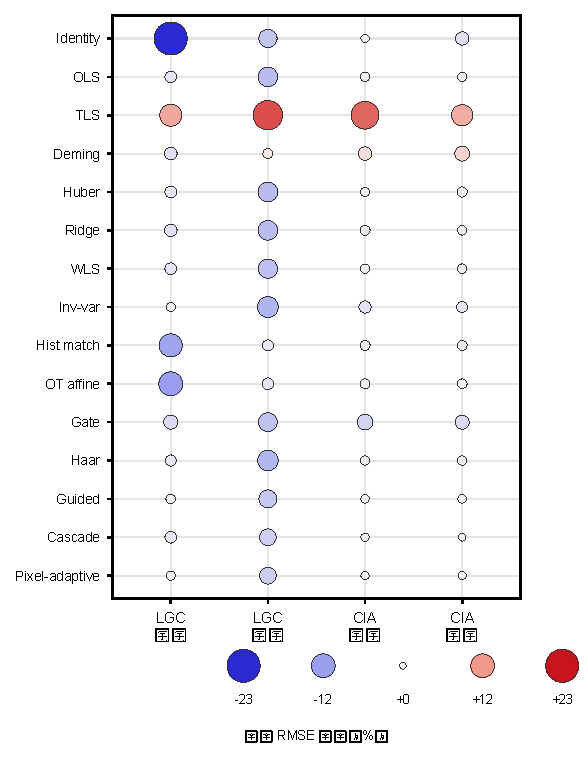
\includegraphics[width=0.94\linewidth]{fig2_gain_matrix_zh.pdf}
\caption{四个划分上十五种已展示校正变体。蓝表示改善、红表示退化；扩展配置含按划分变化的强度，与固定强度主表分别解释。}
\label{fig:gain}
\end{figure}

\subsection{校准诊断说明什么}
稳定期精细与粗糙变化的拟合斜率为 $a=0.544$、$R^2=0.278$；预测的对应值为 $a=0.473$、$R^2=0.202$。骨干已复现相当部分的线性幅度衰减，剩余关系的弱可预测性使逐样本拟合易受方差影响，由此启发观测锚定。这些相关量支持诊断，但不构成不可约信息上限或传感器因果解释的证明。

图~\ref{fig:gain} 显示，校正收益随 regime 与配置改变。重训骨干的稳定期比较中，OLS 退化 9.6\%，替换改善 13.5\%。因此，校准的作用同时依赖观测和底层预测。

\subsection{训练未消除划分间权衡}
\begin{table}[t]
\centering
\caption{九骨干评测。RMSE 于 $[0,1]$；SSIM 保留原 $[-1,1]$ 输入域，不与修正后的指标口径混用。}
\label{tab:backbones}
\setlength{\tabcolsep}{2.5pt}
\begin{tabular}{lcccc}
\toprule
 & \multicolumn{2}{c}{稳定期（验证）} & \multicolumn{2}{c}{洪水期（测试）}\\
\cmidrule(lr){2-3}\cmidrule(lr){4-5}
骨干 & RMSE & SSIM & RMSE & SSIM\\
\midrule
Base & \textbf{0.02329} & 0.8918 & 0.02160 & 0.8683\\
+低频损失 & 0.02448 & 0.8895 & 0.02104 & 0.8727\\
+高频损失 & 0.02415 & 0.8959 & 0.02083 & 0.8762\\
+逐波段权重 & 0.02424 & 0.8913 & 0.02122 & 0.8702\\
+差分监督 & 0.02491 & 0.8434 & 0.02450 & 0.8181\\
架构：组合 & 0.02602 & 0.8932 & 0.02334 & 0.8722\\
架构：差分 & 0.02522 & 0.8917 & \textbf{0.02063} & 0.8743\\
架构：门控 & 0.02488 & 0.8922 & 0.02123 & 0.8755\\
架构：重注入 & 0.02559 & 0.8885 & 0.02160 & 0.8722\\
\bottomrule
\end{tabular}
\end{table}

没有训练变体同时改善两个 LGC 划分（表~\ref{tab:backbones}）。显式差分获得最低洪水期 RMSE，但所有变体的稳定期 RMSE 均退化。差分监督改善内部固定噪声验证曲线，却损害独立报告的得分，提示必须控制验证噪声敏感性。

训练后的门控在一百个噪声级上均接近 $g(t)=0.622$，原本的时间依赖信任机制表现为常数缩放。这是一项具体负面结果，不能外推为任何训练目标都无法学习可靠性。

\begin{figure}[t]
\centering
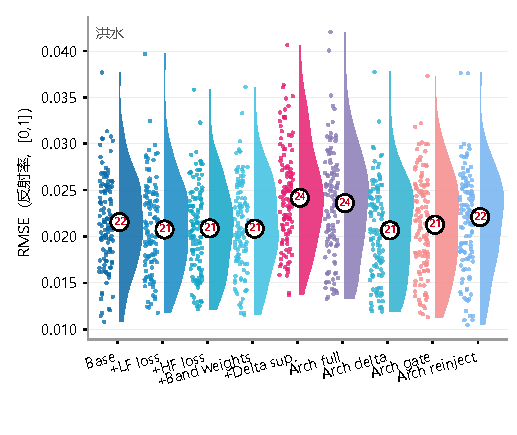
\includegraphics[width=\linewidth]{fig1_raincloud_zh.pdf}
\caption{九骨干的洪水期逐 patch RMSE：点为 patch，半小提琴为密度，圆标为中位数（$\times10^{-3}$）。这些是模型变体，不是重复训练种子。}
\label{fig:rain}
\end{figure}

\subsection{组合系统与计算开销}
\begin{table}[t]
\centering
\caption{组合系统比较，RMSE 于 $[0,1]$。组合系统为重训骨干加低频替换，$\lambda=0.3$。}
\label{tab:system}
\setlength{\tabcolsep}{2.5pt}
\begin{tabular}{lcccc}
\toprule
 & \multicolumn{2}{c}{LGC} & \multicolumn{2}{c}{CIA}\\
\cmidrule(lr){2-3}\cmidrule(lr){4-5}
方法 & 稳定期 & 洪水期 & 验证 & 测试\\
\midrule
历史十步 & 0.02972 & 0.02161 & \textbf{0.02716} & 0.02777\\
Fixed-1 & 0.02815 & 0.02053 & 0.02785 & 0.02741\\
组合系统 & \textbf{0.02014} & \textbf{0.02044} & 0.02846 & \textbf{0.02664}\\
\bottomrule
\end{tabular}
\end{table}

组合系统的 LGC 稳定期 RMSE 为 0.02014，比历史十步得分低 32.2\%，比仅做替换低 16.6\%。它也优于十步对照的洪水期与 CIA 测试得分，但损害 CIA 验证期（表~\ref{tab:system}）。仅做替换的洪水期与 CIA 测试误差仍更低，因此重训增加的是稳定期收益，而非全面改善。

替换仅需一次网络评估（NFE）与可分离滤波，迭代对照为十次。历史 CPU 测量为每 patch 0.93\,s 对 4.65\,s，实测约加速五倍；网络调用减少十倍不等于墙钟时间加速十倍。

\balance
\section{结论}
\label{sec:concl}
观测锚定低频替换为单步扩散 STF 提供了简洁校正。历史比较同时呈现 LGC 增益、CIA 验证期失败及九骨干未能化解的划分间权衡；线性变化诊断与门控坍缩进一步限定了机制解释。最终性能主张仍需匹配采样设置、修正指标、多训练种子和同协议外部对比。

\bibliographystyle{IEEEbib}
\bibliography{refs}
\end{document}
